\documentclass[conference]{IEEEtran}
\IEEEoverridecommandlockouts

\usepackage{cite}
\usepackage{amsmath,amssymb,amsfonts}
\usepackage{graphicx}
\usepackage{textcomp}
\usepackage{xcolor}
\usepackage{booktabs}
\usepackage{array}
\usepackage{microtype}
\usepackage{tikz}
\usetikzlibrary{arrows.meta, positioning, calc}
\usepackage{hyperref}
\hypersetup{colorlinks=true, linkcolor=blue!50!black, citecolor=blue!50!black, urlcolor=blue!50!black}

\emergencystretch=2em

\begin{document}

\title{AI\,--\,Collective: A Ports-and-Adapters Core\\for Configurable Multi-Agent LLM Orchestration}

\author{
\IEEEauthorblockN{SuZeAI (SuzeNith)}
\IEEEauthorblockA{\textit{Independent Researcher} \\
\texttt{suzeai545@gmail.com} \\
\url{https://github.com/SuZeAI/ai-collective}}
}

\maketitle

\begin{abstract}
We describe the core of AI\,--\,Collective, an open, source-available
system for running large language model (LLM) agents individually or as
coordinated multi-agent systems. The core is organized as a
ports-and-adapters (hexagonal) codebase: a framework-free domain layer
defines the orchestration logic, an application layer exposes it through
provider-agnostic Protocols, and an infrastructure layer supplies concrete
adapters for LLM providers, storage, task queues, and distributed locks. On
top of this, six LangGraph-based orchestration topologies (sequential,
ring, supervisor, tree, mesh, and a user-defined custom graph) share a
common runtime that bounds recursion, tolerates partial failure, and
absorbs transient provider errors. A three-tier memory subsystem
(per-turn context, a per-conversation knowledge graph, and a
scope-isolated long-term memory store) and a sixteen-stage LLM middleware
stack (loop detection, retries, prompt caching, cost budgeting, guardrails)
are applied uniformly to every agent call. We present the core's
layering, its orchestration and memory internals, its middleware
composition strategy, and its security controls (SSRF protection, JWT
hardening, sandboxed tool execution), and discuss the design trade-offs
that follow from targeting deployments ranging from a single laptop to a
distributed Kubernetes cluster from one codebase.
\end{abstract}

\begin{IEEEkeywords}
multi-agent systems, large language models, LLM orchestration, LangGraph,
hexagonal architecture, agent memory, tool use, core architecture
\end{IEEEkeywords}

\section{Introduction}

Serving an LLM as a multi-turn, tool-using agent -- and, further, as a
member of a coordinated group of agents -- places different demands on a
system than serving a stateless completion endpoint. The core must
choose a communication topology among agents, bound and recover from
long-running or failing model/tool calls, manage memory at more than one
time scale, and remain portable across LLM providers and infrastructure
tiers without becoming entangled with any one of them.

This paper documents the \emph{core} of AI\,--\,Collective: the component
that implements this functionality. We deliberately scope the paper to
that core: the orchestration runtime, memory subsystem, middleware stack, and
the ports-and-adapters layering that keeps them independent of any
concrete LLM vendor or infrastructure choice. Client-facing concerns are
out of scope.

The remainder of the paper is organized as follows.
Section~\ref{sec:related} situates the work relative to existing
multi-agent frameworks. Section~\ref{sec:architecture} describes the
core's layered architecture. Section~\ref{sec:orchestration} details the
multi-agent orchestration runtime. Section~\ref{sec:memory} describes the
memory subsystem. Section~\ref{sec:middleware} describes the LLM
middleware stack. Section~\ref{sec:tools} covers tool execution and
sandboxing. Section~\ref{sec:deployment} covers storage/queue/lock
elasticity. Section~\ref{sec:security} covers the security model.
Section~\ref{sec:limitations} discusses limitations, and
Section~\ref{sec:conclusion} concludes.

\section{Related Work}
\label{sec:related}

AutoGen~\cite{autogen} generalizes single-user/assistant chat into
programmable conversation among configurable agents. MetaGPT~\cite{metagpt}
assigns agents fixed software-engineering roles that communicate through
structured document artifacts. CrewAI~\cite{crewai} offers a
process-oriented ``crew of agents with roles and tasks'' abstraction.
LangGraph~\cite{langgraph}, on which this core's execution layer is
built, provides a lower-level primitive: agents and control flow are
represented explicitly as nodes and edges in a state graph, with
first-class persistence, streaming, and human-in-the-loop interrupts.

The AI\,--\,Collective core sits above LangGraph and contributes what
these frameworks typically leave to the integrator: (1) a fixed catalogue
of \emph{selectable} topologies for common collaboration patterns, with an
explicit escape hatch to a fully custom graph; (2) a hexagonal layering
that keeps orchestration logic independent of the concrete LLM provider,
persistence engine, task queue, and lock implementation; and (3) a
uniformly applied middleware stack that turns reliability and cost
controls (loop detection, retries, budgets) into cross-cutting,
declaratively configured behavior rather than per-agent boilerplate.

\section{Core Architecture}
\label{sec:architecture}

The core follows a ports-and-adapters (hexagonal) layering with
dependencies pointing strictly inward:

\begin{center}
\footnotesize
\begin{tabular}{@{}ll@{}}
\toprule
\textbf{Package} & \textbf{Responsibility} \\
\midrule
\texttt{api/}    & FastAPI app, routers, schemas, DI, auth \\
\texttt{app/}    & Use-case services; \texttt{ports/} holds Protocols \\
\texttt{domain/} & Framework-free business logic, dataclass models \\
\texttt{infra/}  & Adapters implementing \texttt{app.ports} \\
\texttt{share/}  & Small cross-layer utilities (logging, text) \\
\bottomrule
\end{tabular}
\end{center}

\texttt{domain} imports nothing from \texttt{app}, \texttt{api}, or
\texttt{infra}. \texttt{app} depends only on Protocols declared in
\texttt{app/ports/} (\texttt{repositories.py}, \texttt{llm.py},
\texttt{staff\_graph.py}, \texttt{security.py}) and never on a concrete
adapter. \texttt{infra} supplies the implementations -- JSON-file or
MongoDB repositories, LangChain-based LLM provider adapters, RabbitMQ or
in-memory task queues, Redis or threading locks, local or Kubernetes
sandboxes. \texttt{api/deps.py} is the composition root: it wires concrete
adapters into application services through FastAPI's dependency-injection
system. Domain-level errors are translated to HTTP status codes by
exception handlers registered centrally, so neither the domain nor the
application layer constructs an HTTP response directly.

A request is handled in four steps: (1) FastAPI routes it to a handler in
\texttt{api/routers/}; (2) a \texttt{Depends(...)} factory builds the
relevant service with its injected repositories and LLM provider; (3) the
service runs the use case against domain logic and ports; (4) domain
errors are mapped to HTTP responses by handlers in \texttt{api/main.py}.
This strict separation is what allows Sections~\ref{sec:orchestration}
through~\ref{sec:deployment} to describe orchestration, memory, and
infrastructure choice independently: none of them can leak into the
others through an import.

\begin{figure}[t]
\centering
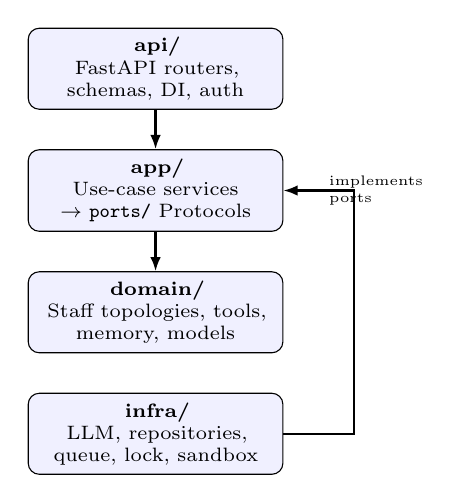
\begin{tikzpicture}[
    node distance=5mm,
    box/.style={draw, rounded corners, align=center, minimum height=7mm,
        text width=3.0cm, fill=blue!6, font=\scriptsize},
    arr/.style={-{Latex[length=1.8mm]}, thick}
]
\node[box] (api) {\textbf{api/}\\FastAPI routers, schemas, DI, auth};
\node[box, below=of api] (app) {\textbf{app/}\\Use-case services $\rightarrow$ \texttt{ports/} Protocols};
\node[box, below=of app] (domain) {\textbf{domain/}\\Staff topologies, tools, memory, models};
\node[box, below=of domain] (infra) {\textbf{infra/}\\LLM, repositories, queue, lock, sandbox};

\draw[arr] (api) -- (app);
\draw[arr] (app) -- (domain);
\draw[arr] (infra.east) -- ++(0.9,0) |- node[pos=0.75, right, font=\tiny, align=left] {implements\\ports} (app.east);
\end{tikzpicture}
\caption{Core layering. \texttt{domain} depends on nothing outward;
\texttt{app} depends only on \texttt{ports} Protocols; \texttt{infra}
implements those Protocols and is wired in by \texttt{api/deps.py}.}
\label{fig:layers}
\end{figure}

\section{Multi-Agent Orchestration Runtime}
\label{sec:orchestration}

Multi-agent execution is implemented in \texttt{domain/staff/} as six
LangGraph state machines, selected at request time via
\texttt{api/deps.get\_staff\_graph\_service(mode=...)}. Each topology
exposes a blocking \texttt{run(...)} and a streaming
\texttt{run\_stream(...)}, both accepting the user input, the participating
agent definitions, an \texttt{LLMProvider}, a round bound, and an optional
knowledge-graph context provider.

\begin{center}
\footnotesize
\begin{tabular}{@{}l>{\raggedright\arraybackslash}p{6.4cm}@{}}
\toprule
\textbf{Mode} & \textbf{Behavior} \\
\midrule
sequential & One agent processes the request in a single pass (default). \\
ring & Agents take turns in a fixed circular order until a round bound; each turn sees full history. \\
supervisor & A lead agent delegates to workers via an inline control tag and synthesizes their replies. \\
tree & Agents are arranged as a parent/child tree; results roll up leaves-to-root. \\
mesh & A hub agent selects among $N$ spokes via control tags (\texttt{<NEXT\_AGENT>}, \texttt{<DISCUSSION\_END>}). \\
custom & A user-defined LangGraph DAG (\texttt{CustomGraphSpec}). \\
\bottomrule
\end{tabular}
\end{center}

\subsection{Shared runtime guarantees}

All six topologies build on \texttt{\_graph\_runtime.py}, which supplies
three properties:

\begin{itemize}
    \item \textbf{Bounded recursion.} \texttt{recursion\_config(max\_rounds)}
    sets the LangGraph recursion limit to
    $\max(25,\ 2\cdot\mathtt{max\_rounds}+10)$, so legitimately long runs
    do not trip the default 25-superstep ceiling while worst-case
    execution remains bounded.
    \item \textbf{Graceful degradation.} \texttt{run\_to\_final\_state}
    streams the graph in values mode and, if the recursion limit is hit or
    a node raises, returns the \emph{latest partial state} instead of
    discarding the run.
    \item \textbf{Resilient model calls.} \texttt{safe\_chat} wraps every
    \texttt{llm.chat} call with a bounded timeout and retry/backoff; on
    exhaustion it substitutes an error string for that turn rather than
    aborting the run.
\end{itemize}

A further invariant holds across all six implementations: LangGraph state
is never mutated in place. Extending a collection in state (e.g.\
\texttt{conversation\_history}) requires building a new container, which
LangGraph's checkpointing and state-diffing depend on.

\subsection{Token budgeting and subagents}

\texttt{token\_budget.py} trims per-turn context to
\texttt{staff.context\_token\_limit} minus
\texttt{staff.output\_token\_reserve}; this estimate covers system- and
user-authored text only and does not account for bound tool-schema tokens.
Beyond the six topologies, an individual agent's tool loop may spawn
\emph{subagents} (\texttt{subagents.py}) bounded by
\texttt{subagent\_max\_concurrent} and \texttt{subagent\_max\_turns} for
parallel task delegation; subagents may be granted sandboxed tools, with
the sandbox (Section~\ref{sec:tools}) as the enforced security boundary.

\section{Memory Subsystem}
\label{sec:memory}

The core separates memory into three tiers of increasing durability.

\subsection{Working memory and knowledge graph}

Within one conversation, turns are ingested into a knowledge graph
(\texttt{domain/memory/}) that extracts entities and relationships using
either a rule-based \texttt{static} extractor (spaCy) or an
\texttt{llm}-based extractor, selected by \texttt{graph.build\_mode}. This
graph is scoped to a single \texttt{conversation\_id}.

\subsection{Long-term memory}

Long-term memory (LTM) persists facts, preferences, and episodic notes
\emph{across} tasks. It is off by default, in which case the core
behaves as if it did not exist. Each record is scoped along three
independent dimensions -- \texttt{company\_id}, \texttt{owner\_id},
\texttt{staff\_id} -- any of which may be unset (``applies broadly''); a
recall query matches records that are equal-or-broader on every
dimension, so isolation between users and agents holds regardless of
scope breadth. Isolation is enforced both client-side (brute-force/FAISS
scoring) and server-side (a Qdrant payload filter), so the guarantee does
not depend on which vector-store adapter is active.

Two operations drive LTM, both implemented as LLM middleware
(Section~\ref{sec:middleware}): \textbf{recall} injects a scoped digest as
a system message before every model call, and \textbf{consolidation}, on a
clean run finish, promotes salient short-term notes into LTM with
near-duplicate deduplication. Recall scoring blends semantic similarity
(dense cosine, when embeddings are enabled) with importance and
recency, falling back to lexical term overlap otherwise. The embedding
provider is itself pluggable (\texttt{infra/llm/embeddings.py}) -- a
dependency-free hashing embedder by default, or Google/OpenAI/OpenAI-compatible
embeddings -- mirroring the LLM provider abstraction. An optional
approximate-nearest-neighbor index (FAISS locally, Qdrant as an external
service, both under \texttt{infra/vector\_store/}) replaces the default
brute-force cosine scan at scale; if the index is unavailable or returns
nothing, recall transparently falls back to brute force.

\section{LLM Middleware Stack}
\label{sec:middleware}

The LLM provider's \texttt{chat()} (\texttt{infra/llm/}) delegates to
LangChain's \texttt{create\_agent} rather than a hand-rolled ReAct loop,
and every cross-cutting concern is expressed as composable middleware,
assembled by \texttt{build\_default\_middleware()}
(\texttt{infra/llm/middleware/builder.py}) and applied to every agent in
every topology. Each middleware hooks either tool execution
(\texttt{awrap\_tool\_call}) or the model call
(\texttt{before\_model}/\texttt{after\_model}).

\begin{table}[t]
\centering
\footnotesize
\caption{Default middleware stack, in composition order.}
\label{tab:middleware}
\begin{tabular}{@{}clll@{}}
\toprule
\# & Middleware & Hook & Default \\
\midrule
1  & ModelCallLimit          & model & on \\
2  & ToolCallLimit           & tool  & off \\
3  & Guardrail               & tool  & off \\
4  & ToolResultCache         & tool  & off \\
5  & LoopDetection           & tool  & \textbf{on} \\
6  & ToolRetry               & tool  & \textbf{on} (2$\times$) \\
7  & ToolTimeout             & tool  & on \\
8  & PIIRedaction            & tool  & off \\
9  & AnthropicPromptCaching  & model & off (Anthropic only) \\
10 & ModelFallback           & model & off \\
11 & ModelRetry              & model & off \\
12 & ContextEditing          & model & off \\
13 & Summarization           & model & off \\
14 & RollingSummary          & model & off \\
15 & LongTermMemory          & model & off \\
16 & CostBudget              & model & off \\
\bottomrule
\end{tabular}
\end{table}

The order (Table~\ref{tab:middleware}) is deliberate: guardrail and
PII-redaction protect tool execution before it happens; the result cache
is checked before retry/timeout do real work; loop-detection, retry, and
timeout wrap the tool call itself; and the model-facing group -- trim
history, recall long-term memory, enforce a cost budget -- acts around the
model call. \textbf{LoopDetection}, on by default, detects an agent
re-issuing an identical tool call (same name and arguments) a configurable
number of times and nudges it to change approach or finalize, without
hard-aborting the run. \textbf{AnthropicPromptCaching} marks the system
prompt, tool definitions, and last-message prefix as cacheable so repeated
calls sharing that prefix -- agent-loop rounds, ring/sequential hops,
subagent fan-out -- are served from provider-side cache; it is a strict
prefix match, so any earlier byte-level change invalidates the cache for
everything after it, and it is a silent no-op on non-Anthropic providers.

\section{Tool Execution and Sandboxing}
\label{sec:tools}

Capabilities beyond text generation are exposed as tool implementations in
\texttt{domain/tools/}, bound per-agent rather than hard-coded into a
role. Code-execution tools (Bash, Python) run through a
\texttt{SandboxProvider} (\texttt{infra/sandbox/}) with two modes: a local
subprocess on the host machine, suited to development, or a
per-request Kubernetes pod spawned by a dedicated provisioner service for
production isolation with automatic lifecycle management. Outbound-request
tools (HTTP client, browser navigation) are routed through an SSRF guard
(Section~\ref{sec:security}) rather than trusting tool-supplied URLs
directly.

\section{Storage, Queueing, and Locking Elasticity}
\label{sec:deployment}

Three infrastructure concerns are each abstracted behind an
\texttt{app/ports} Protocol and selected purely by configuration:

\begin{itemize}
    \item \textbf{Storage} (\texttt{infra/repositories/}) -- JSON files
    loaded into memory and rewritten on update (default; adequate for
    small/medium datasets), or MongoDB via the async Motor driver.
    \item \textbf{Task queue} (\texttt{infra/task\_queue.py}) -- an
    in-process \texttt{ThreadPoolExecutor} by default, or RabbitMQ to
    detach long-running runs onto distributed workers.
    \item \textbf{Distributed lock} (\texttt{infra/lock\_provider.py}) -- a
    threading lock by default, or Redis when staff-graph transitions must
    be mutually excluded across multiple concurrently running processes.
\end{itemize}

This three-axis elasticity, combined with the local/Kubernetes sandbox
choice (Section~\ref{sec:tools}), lets one deployable image serve both a
single-laptop evaluation deployment and a horizontally scaled,
multi-tenant production deployment without a code change.

\section{Security Model}
\label{sec:security}

Because bound tools can make outbound network requests, execute code, and
act on third-party accounts, several controls are enforced at the
framework level rather than left to individual tool implementations.

\textbf{Authentication.} Passwords are hashed with bcrypt
(\texttt{api/security.py}); sessions use HS256-signed JWT access tokens
validated on every request. In production
(\texttt{ENVIRONMENT=production}), startup fails fast if the JWT signing
secret is the placeholder default or shorter than 32 bytes.

\textbf{SSRF protection.} Any tool capable of fetching an arbitrary URL is
routed through a guard (\texttt{domain/tools/\_ssrf.py}) that restricts
schemes to \texttt{http}/\texttt{https}, resolves the hostname and rejects
addresses that are private, loopback, link-local, reserved, multicast, or
unspecified -- blocking cloud metadata endpoints and internal services --
and re-validates the target of every redirect to prevent
redirect-based SSRF bypass.

\textbf{Webhook verification.} Inbound platform webhooks
(\texttt{domain/third\_party/}) are authenticated per-platform before any
processing; XML ingestion is parsed with \texttt{defusedxml} to prevent
XXE and billion-laughs payloads.

\textbf{Secret hygiene.} Sensitive dataclass fields (password hashes,
OAuth provider identifiers) are excluded from Python's automatic
\texttt{repr}, so a logged object or unhandled traceback cannot leak a
credential.

\section{Limitations and Future Work}
\label{sec:limitations}

Token budgeting accounts only for system- and user-authored text, not for
the schema size of bound tools, which can understate context pressure for
agents with many tools attached. Delegation in the supervisor, tree, and
mesh topologies relies on inline text control tags rather than a
structured, provider-native function-call channel, trading provider
portability for text-parsing robustness. The default JSON storage adapter
loads each collection into memory and rewrites it on update, adequate for
small/medium datasets but not intended to scale without migrating to the
MongoDB adapter. A quantitative evaluation of topology choice versus task
outcome quality, latency, and cost, and a systematic red-team evaluation
of the prompt-injection surface introduced by tool-bearing subagents, are
left to future empirical work.

\section{Conclusion}
\label{sec:conclusion}

The AI\,--\,Collective core shows that a multi-agent LLM orchestration
system can be built with the same architectural discipline as
conventional software systems: strict hexagonal separation between
orchestration logic and concrete providers/infrastructure, a small set of
well-defined communication topologies rather than unconstrained
agent-to-agent messaging, and a memory and middleware model that treats
reliability -- bounded recursion, partial-failure tolerance, loop
detection, cost budgeting -- as a first-class, uniformly applied concern.
The resulting provider-, storage-, queue-, and lock-agnostic design lets
one codebase serve both local experimentation and distributed production
deployment.

\begin{thebibliography}{9}

\bibitem{langgraph}
LangChain AI, ``LangGraph: Build resilient language agents as graphs,''
\url{https://github.com/langchain-ai/langgraph}, 2024.

\bibitem{autogen}
Q.~Wu, G.~Bansal, J.~Zhang, Y.~Wu, S.~Zhang, E.~Zhu, B.~Li, L.~Jiang,
X.~Zhang, and C.~Wang, ``AutoGen: Enabling Next-Gen LLM Applications via
Multi-Agent Conversation,'' \emph{arXiv:2308.08155}, 2023.

\bibitem{metagpt}
S.~Hong, X.~Zheng, J.~Chen, Y.~Cheng, J.~Wang, C.~Zhang, Z.~Wang,
S.~K.~S.~Yau, Z.~Lin, L.~Zhou, C.~Ran, L.~Xiao, C.~Wu, and J.~Schmidhuber,
``MetaGPT: Meta Programming for a Multi-Agent Collaborative Framework,''
\emph{arXiv:2308.00352}, 2023.

\bibitem{crewai}
J.~Moura et al., ``CrewAI: Framework for orchestrating role-playing,
autonomous AI agents,'' \url{https://github.com/crewAIInc/crewAI}, 2024.

\end{thebibliography}

\end{document}
